\documentclass[crop,tikz,convert={outext=.svg,command=\unexpanded{pdf2svg \infile\space\outfile}},multi=false]{standalone}
\usepackage{tikz}
\usepackage{pgfplots}
\usetikzlibrary{calc}

\begin{document}
    \begin{center}
        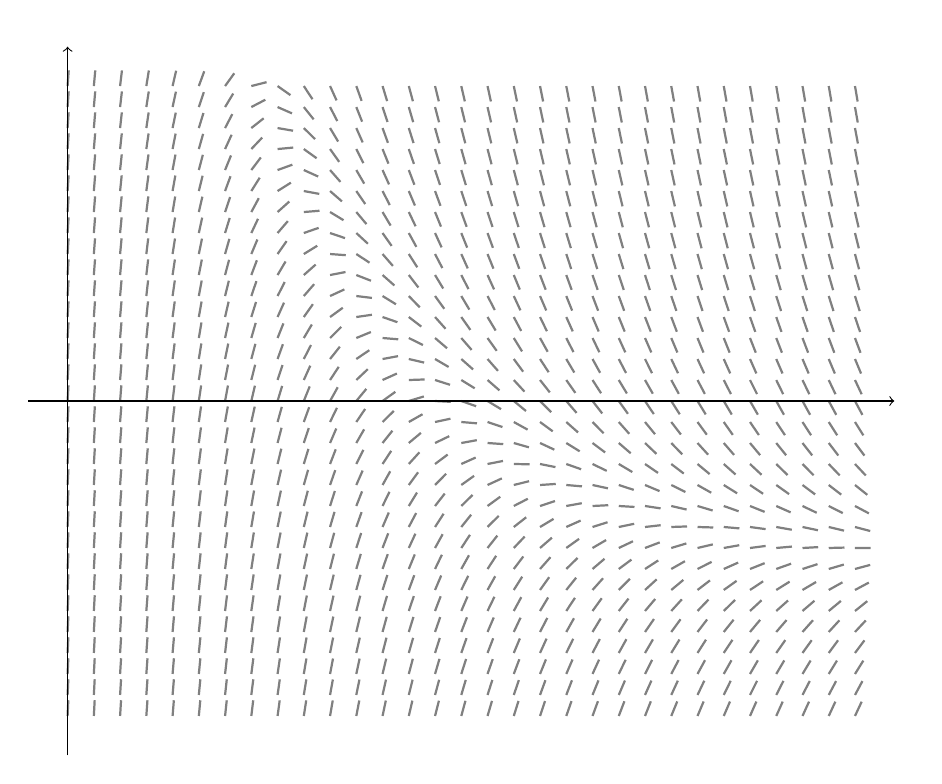
\begin{tikzpicture}[declare function={f(\x,\y)=exp(3-\x/2)-\y-2;}]
            \def\xmax{10} \def\xmin{0}
            \def\ymax{4} \def\ymin{-4}
            \def\nx{30}
            \def\ny{30}

            \pgfmathsetmacro{\hx}{(\xmax-\xmin)/\nx}
            \pgfmathsetmacro{\hy}{(\ymax-\ymin)/\ny}
            \foreach \i in {0,...,\nx}
            \foreach \j in {0,...,\ny}{
                \pgfmathsetmacro{\yprime}{f({\xmin+\i*\hx},{\ymin+\j*\hy})}
                \draw[gray,thick,shift={({\xmin+\i*\hx},{\ymin+\j*\hy})}] 
                (0,0)--($(0,0)!2mm!(.1,.1*\yprime)$);
            }
            \def\yo{1}

            \draw[->] (\xmin-.5,0)--(\xmax+.5,0) node[below right] {};
            \draw[->] (0,\ymin-.5)--(0,\ymax+.5) node[above left] {};
        \end{tikzpicture}
    \end{center}

\end{document}